\documentclass{article}

%\usepackage{showframe}

\usepackage{amsmath}
\usepackage{amsfonts}
\usepackage{amssymb}
\usepackage{amsthm}
\usepackage{diagbox}
\usepackage{graphicx}
\usepackage[hidelinks]{hyperref}
\usepackage{enumitem}
\usepackage{eucal}
\usepackage{algorithm}
\usepackage{algpseudocode}
\usepackage{bm}
\usepackage{bbm}
\usepackage{multirow}
%\usepackage[inline]{showlabels}
%\renewcommand{\showlabelfont}{\tiny\sffamily}
\usepackage{mathtools}
\DeclarePairedDelimiter{\ceil}{\lceil}{\rceil}
\DeclarePairedDelimiter{\floor}{\lfloor}{\rfloor}
\DeclareMathOperator*{\argmax}{argmax}
\DeclareMathOperator*{\argmin}{argmin}
\usepackage{etoolbox}
\usepackage{tikz}
\usetikzlibrary{arrows}

% "draft" stuff here
\usepackage{lineno}
\linenumbers%
\usepackage{setspace}
\usepackage{subcaption}


\newtheorem{alg}{Algorithm}
\newtheorem{defn}{Definition}
\newtheorem{lem}{Lemma}
\newtheorem{obs}{Observation}
\newtheorem{prob}{Problem}
\newtheorem{prop}{Proposition}
\newtheorem{thm}{Theorem}
\newtheorem{cor}{Corollary}

%% Patch 'normal' math environments:
\newcommand*\linenomathpatch[1]{%
  \cspreto{#1}{\linenomath}%
  \cspreto{#1*}{\linenomath}%
  \csappto{end#1}{\endlinenomath}%
  \csappto{end#1*}{\endlinenomath}%
}

\linenomathpatch{equation}
\linenomathpatch{gather}
\linenomathpatch{multline}
\linenomathpatch{align}
\linenomathpatch{alignat}
\linenomathpatch{flalign}

\newcommand{\E}{\mathbb{E}}
\newcommand{\IndexToChild}{\textsf{IndexToChild}}
\newcommand{\ParentToRange}{\textsf{ParentToRange}}
\newcommand{\Rotate}{\textsf{Rotate}}
\newcommand{\bP}{\mathbf{P}}
\newcommand{\PP}{\mathbb{P}}
\newcommand{\bY}{\mathbf{Y}}
\newcommand{\bet}{\boldsymbol{\eta}}
\newcommand{\bphi}{\boldsymbol{\phi}}
\newcommand{\bpi}{\boldsymbol{\pi}}
\newcommand{\bpmarg}{\breve{\mathbf{p}}}
\newcommand{\bp}{\mathbf{p}}
\newcommand{\brmarg}{\breve{\mathbf{r}}}
\newcommand{\br}{\mathbf{r}}
\newcommand{\bq}{\mathbf{q}}
\newcommand{\bs}{\mathbf{s}}
\newcommand{\bpsi}{\boldsymbol{\psi}}
\newcommand{\btheta}{\boldsymbol{\theta}}
\newcommand{\bt}{\mathbf{t}}
\newcommand{\bu}{\mathbf{u}}
\newcommand{\cT}{\mathcal{T}}
\newcommand{\Q}{\mathbf{Q}}
\newcommand{\transpose}{\top}
\newcommand{\leaves}{\mathcal{L}}
\newcommand{\libsbn}{\textsf{libsbn}}
\newcommand{\median}{\operatorname{median}}
\newcommand{\parent}{\mathsf{pa}}
\newcommand{\pcsp}[2]{{#1}\hspace{-0.09em}\rightarrow\hspace{-0.09em}{#2}}
\newcommand{\pcspts}{\pcsp{t}{s}}
\newcommand{\posterior}{p_{\mathrm{post}}}
\newcommand{\prior}{p_{\mathrm{pr}}}
\newcommand{\rotatedleftarrow}{\xleftarrow{\sim}}
\newcommand{\rotatedrightarrow}{\xrightarrow{\sim}}
\newcommand{\rotated}[1]{\tilde{#1}}
\newcommand{\sorted}[1]{\mathring{#1}}
\newcommand{\sdag}{\mathcal{D}}
\newcommand{\topleaf}{\mathcal{T}_{\text{leaf}}}
\newcommand{\toproot}{\mathcal{T}_{\text{root}}}
\newcommand{\upost}{p_{\mathrm{unno}}}
\newcommand{\PPprior}{\PP_{\text{prior}}}
\newcommand{\PPpost}{\PP_{\text{post}}}
\newcommand{\checkell}{\check{\ell}}
\newcommand{\locallike}{\mathfrak{L} }

\newcommand{\sscl}[2]{(#1,\underline{#2})}
\newcommand{\nakedsscl}[2]{#1,\underline{#2}}
\newcommand{\setsscl}[2]{\{#1,\underline{#2}\}}
\newcommand{\subsplit}[2]{\{\{#1\},\{#2\}\}}
\newcommand{\lsc}[1]{\acute{#1}}
\newcommand{\rsc}[1]{\grave{#1}}
\newcommand{\from}{\gets}
\newcommand{\taudown}{\tau^\downarrow}
\newcommand{\tauup}{\tau^\uparrow}

\newcommand{\iqtree}{\texttt{iqtree}}
\newcommand{\bito}{\texttt{bito}}
\newcommand{\beagle}{\texttt{BEAGLE}}
\newcommand{\citet}[1]{\cite{#1}}
\newcommand{\citep}[1]{\cite{#1}}



\newlength{\arrowwidth}
\DeclareRobustCommand{\customrightarrow}{
	\settowidth{\arrowwidth}{$\to$}
	\tikz[baseline=-0.5ex]{\draw [-latex](0,0) --(\arrowwidth,0);}
}

% http://bytesizebio.net/2013/03/11/adding-supplementary-tables-and-figures-in-latex/
\newcommand{\beginsupplement}{%
        \setcounter{table}{0}
        \renewcommand{\thetable}{S\arabic{table}}%
        \setcounter{figure}{0}
        \renewcommand{\thefigure}{S\arabic{figure}}%
     }

\hyphenation{Ge-nome Ge-nomes hyper-mut-ation through-put}

\title{...systematic nni-search...}
\author{%
...authors...}
\date{%
}


\begin{document}
\allowdisplaybreaks

\maketitle

\clearpage


\begin{abstract}
...abstract...
\end{abstract}


% Need to add a lot of references...


\section{Introduction}

Statistical phylogenetics often involve an exploration of tree space and likelihood computations.

Move between topologies with local rearrangements of the tree structure. 
NNIs and SPRs.

Maximum likelihood methods attempt to find the max likehood tree. 
Systematically apply local rearrangements to improve likelihood. 
Tends to be fast, but produces a single tree.

Bayesian methods estimate the posterior distribution on trees. 
Often this is sampling topologies or tree by MCMC methods. 
One sample to the next are related by a local rearrangement, likelihood calculation, then accept or reject. 
High posterior topologies are resampled many times. 
This produces many trees and approximate probabilities, but slow. 
Doesn't scale well.

We want to find the posterior distribution on trees quickly.

Phylogenetic topographer performs a systematic exploration of tree space by local rearrangements of the witnessed topologies and including the resulting topologies above some likelihood threshhold. 
Normalizing the likelihoods of all witnessed topologies gives an approximation of Bayesian posterior distribution. 
Still slow.

The problem is there are too many trees.

The sDAG compactily represents many trees. 
Used for variational approximation, generalized pruning likelihoods and branch lengths, other stuff.

Here we try a systematic search with sDAGs instead of trees.
We will add NNIs to the sDAG like for ML phylogenetics.
For trees, NNIs move from tree to tree.
For sDAGs, NNIs make the sDAG larger.
Exploring tree space with NNIs on trees evaluates quality of NNIs by comparing likelihoods (and priors for Bayesian methods) of trees.
We need a way to evaluate the quality of a NNI enlarging an sDAG.
We propose two ways, which we call generalized pruning and top pruning.

In this article we describe the sDAG structure, NNIs on the sDAG, and our two systematic search algorithms.
Then we see how well they perform by trying them several data sets often used for benchmarking Bayesian phylogenetic methods and compare with MCMC. 
Generalized pruning doesn't look so good.
Top pruning results are promising.





The goal of a systematic search algorithm on subsplit DAGs is to find edges to add to the sDAG that cover additional high-posterior regions of tree space.
Our algorithm is modeled after NNI-based exploration of tree space, in which the likelihood for NNI operations are calculated in constant time using partial likelihood vectors.
Rather than finding trees to add to the sDAG, we are finding edges to add to the sDAG.
Specifically, we add sDAG edges and nodes based on NNIs of the sDAG, as described in subsection \ref{subsec:sdag_nni}.
We emphasize that we try to find high-posterior regions of tree space, but we are not trying to determine posterior densities.
Once a region is located by a search method, some other method may be used to infer posterior densities in this region.



\section{Methods}

\subsection{Introduction to the subsplit DAG}
...mostly copied content from subsplit-dag article...

\subsection{Performing NNIs to the subsplit DAG}\label{subsec:sdag_nni}
...mostly copied content from subsplit-dag article...
...explain we associate an NNI to its central edge in the sDAG



\subsection{How do we evaluate new additions to the DAG}\label{subsec:nni_edge_likelihood}

We require a means of calculating a likelihood for an NNI of the sDAG in a way analogous to the calculation of a likelihood for a phylogenetic tree. We take two approaches, described in detail in the following two sections, which we call generalized pruning and top pruning. In both cases the likelihood of the NNI depends on the existing sDAG. Generalized pruning is based on the overall likelihood of the sDAG, while top pruning is based on the likelihood of an individual tree. For the likelihoods, we assume branch lengths are defined on the edges of the sDAG, so that we are computing tree likelihoods rather than topology likelihoods.


\subsubsection{Generalized Pruning}

Generalized pruning tries to add the NNI to an sDAG that most increases the marginal likelihood of trees in the sDAG.
The true marginal likelihood of the trees is
\begin{gather*}
\sum_{\tau\in\mathcal{D}}\prod_{j=1}^K p_{\psi}(Y_k\mid \tau)p(\tau).
\end{gather*}
We have no efficient algorithm for computing this sum and so we make a modification.
Interchanging the summation with the product yields a composite-like marginal likelihood,
\begin{gather}\label{eq:gpLikelihood}
\prod_{j=1}^K\sum_{\tau\in\mathcal{D}} p_{\psi}(Y_k\mid \tau)p(\tau).
\end{gather}
This composite-like marginal likelihood does admit an efficient dynamic programming algorithm. This likelihood was introduced and examined previously \citep{GP}.

% CJS: @Dave, which likelihood do we use in the implementation? 
% Are we using all \tau\in\mathcal{D} or are we restricting down to \tau\in\mathcal{D}_e, where $\mathcal{D_e}$ is the set of trees containing the edge?
% This doesn't matter for maximizing the sum-product likelihood, but it does matter for product-sum likelihood.
% I think we want to restrict down to \tau\in\mathcal{D}_e to limit the effect of topologies in the sDAG that are far away from the edge.
% Other than that, I actually don't know the details for generalized pruning.
% Are we doing the same thing as top pruning, but only the likelihood calculation is different?


\subsubsection{Top Pruning}

Our heuristic for top pruning is that the best addition to an sDAG should introduce the best tree not previously in the sDAG.
We cannot use the true version of this, where we would use a likelihood like
\begin{gather*}
\max_{\tau\in\mathcal{D}_e} \prod_{j=1}^K p_\psi(Y_j\mid \tau)p(\tau)
,
\end{gather*}
and $\mathcal{D}_e$ is the set of trees in the sDAG containing the sDAG edge $e$.
This form would not give an efficient algorithm, as we would need to enumerate all trees and compute their likelihoods.
Instead we store local choices of subtrees, which may yield a sufficient approximation to the tree maximizing the likelihood above.

We define a rootward choice map as a map from each edge of the sDAG to the sister and parent edges that correspond to the best known tree in the sDAG containing that edge.
Similarly, we define a leafward choice map as a map from each edge of the sDAG to the two child edges that correspond to the best known tree containing that edge.
Given these maps we can apply them recursively given a starting edge, filling out a topology.
We can also store branch lengths for every sDAG edge, giving a tree that is ready for likelihood evaluation.
For a given edge, the tree constructed from the choice maps and branch lengths is what we take as the best known tree containing the edge.

To describe the top pruning algorithm and justify the term ``best known tree'', we explain how the choice maps are initialized and maintained.
We assume we start with a tree or trees, coming from a maximum-likelihood tree search, and this tree forms the initial sDAG.
When the initial sDAG is a single tree, the maps and branch lengths are obvious.
To initialize an sDAG from multiple trees, each edge of the sDAG takes its choices and branch lengths from the maximum likelihood input tree that contains the edge.
With multiple input trees, the best known tree for an edge produced by the choice maps need not be one of the input trees.
% CJS: Would a picture here would be helpful? Something illustrating that the best known tree need not be an input tree and also the maps and branch lengths are defined on sDAG edges, not tree edges, which can get confusing.  

Now suppose we are in the situation where we have an sDAG $\mathcal{D}$ with fully defined choice maps and branch lengths.
For an NNI on $\mathcal{D}$ producing $\mathcal{D}^\prime$, a larger sDAG, we must define the choice maps on the edges of $\mathcal{D}^\prime$. 
For edges common to $\mathcal{D}$ and $\mathcal{D}^\prime$, we use the choice maps of $\mathcal{D}$.
There are at most five edges remaining.
Suppose the sDAGs and edges are as depicted in Figure \ref{fig:topPruningChoices}. 
The choice maps and initial values of branch lengths are as follows,
\begin{align}\label{eq:topPruningChoices}
&\text{parent} (u\rightarrow t^\prime)  = \text{parent}(u \rightarrow t),&
&\text{sibling} (u\rightarrow t^\prime) = \text{sibling}(u \rightarrow t),\\\nonumber
&\text{child}_1 (u\rightarrow t^\prime) = t^\prime \rightarrow s^\prime,&
&\text{child}_2 (u\rightarrow t^\prime) = t^\prime \rightarrow Y,\\\nonumber
&\text{branch\_length} (u\rightarrow t^\prime) = \text{branch\_length}(u \rightarrow t),\hspace{-10em}&&\\\nonumber
&\text{parent} (t^\prime\rightarrow s^\prime) = u \rightarrow t^\prime,& 
&\text{sibling} (t^\prime\rightarrow s^\prime) = t^\prime \rightarrow Y,\\\nonumber 
&\text{child}_1 (t^\prime\rightarrow s^\prime) = s^\prime \rightarrow X,& 
&\text{child}_2 (t^\prime\rightarrow s^\prime) = s^\prime \rightarrow Z,\\\nonumber 
&\text{branch\_length} (t^\prime\rightarrow s^\prime) = \text{branch\_length}(t \rightarrow s),\hspace{-10em}&&\\\nonumber
&\text{parent} (t^\prime\rightarrow Y) = u \rightarrow t^\prime,&
&\text{sibling} (t^\prime\rightarrow Y) = t^\prime \rightarrow s^\prime,\\\nonumber
&\text{child}_1 (t^\prime\rightarrow Y) = \text{child}_1(s \rightarrow Y),&
&\text{child}_2 (t^\prime\rightarrow Y) = \text{child}_2(s \rightarrow Y),\\\nonumber
&\text{branch\_length} (t^\prime\rightarrow Y) = \text{branch\_length}(s \rightarrow Y),\hspace{-10em}&&\\\nonumber
&\text{parent} (s^\prime\rightarrow X) = t^\prime \rightarrow s^\prime,&
&\text{sibling} (s^\prime\rightarrow X) = s^\prime \rightarrow Z,\\\nonumber
&\text{child}_1 (s^\prime\rightarrow X) = \text{child}_1(s \rightarrow X),&
&\text{child}_2 (s^\prime\rightarrow X) = \text{child}_2(s \rightarrow X),\\\nonumber
&\text{branch\_length} (s^\prime\rightarrow X) = \text{branch\_length}(s \rightarrow X),\hspace{-10em}&&\\\nonumber
&\text{parent} (s^\prime\rightarrow Z) = t^\prime \rightarrow s^\prime,&
&\text{sibling} (s^\prime\rightarrow Z) = s^\prime \rightarrow X,\\\nonumber 
&\text{child}_1 (s^\prime\rightarrow Z) = \text{child}_1(t \rightarrow Z),&
&\text{child}_2 (s^\prime\rightarrow Z) = \text{child}_2(t \rightarrow Z),\\\nonumber
&\text{branch\_length} (s^\prime\rightarrow Z) = \text{branch\_length}(t\rightarrow Z).\hspace{-10em}&&
\end{align}
In equation \eqref{eq:topPruningChoices}, there is a slight abuse of notation: edges ending in $X$, $Y$, or $Z$
mean edges ending in the root subsplit of $X$, $Y$, or $Z$ respectively.
We emphasize that for edges common to $\mathcal{D}$ and $\mathcal{D}^\prime$, we use the values
from $\mathcal{D}$, not those in equation \eqref{eq:topPruningChoices}.

In summary, given a pre-NNI sDAG with defined choice maps, we extend the choice maps to the post-NNI sDAG.
For the branch lengths, we use those in equation \eqref{eq:topPruningChoices} as starting values for optimization. 
We optimize these branch lengths to maximize the likelihood of the best known tree associated to the NNI.
For edges present in $\mathcal{D}$, the branch lengths are unaltered.
The edge $t^\prime\rightarrow s^\prime$ of $\mathcal{D}^\prime$ has a well-defined best known tree.
We define the likelihood of the NNI to be the likelihood of this tree. 

\begin{figure}[!th]\centering
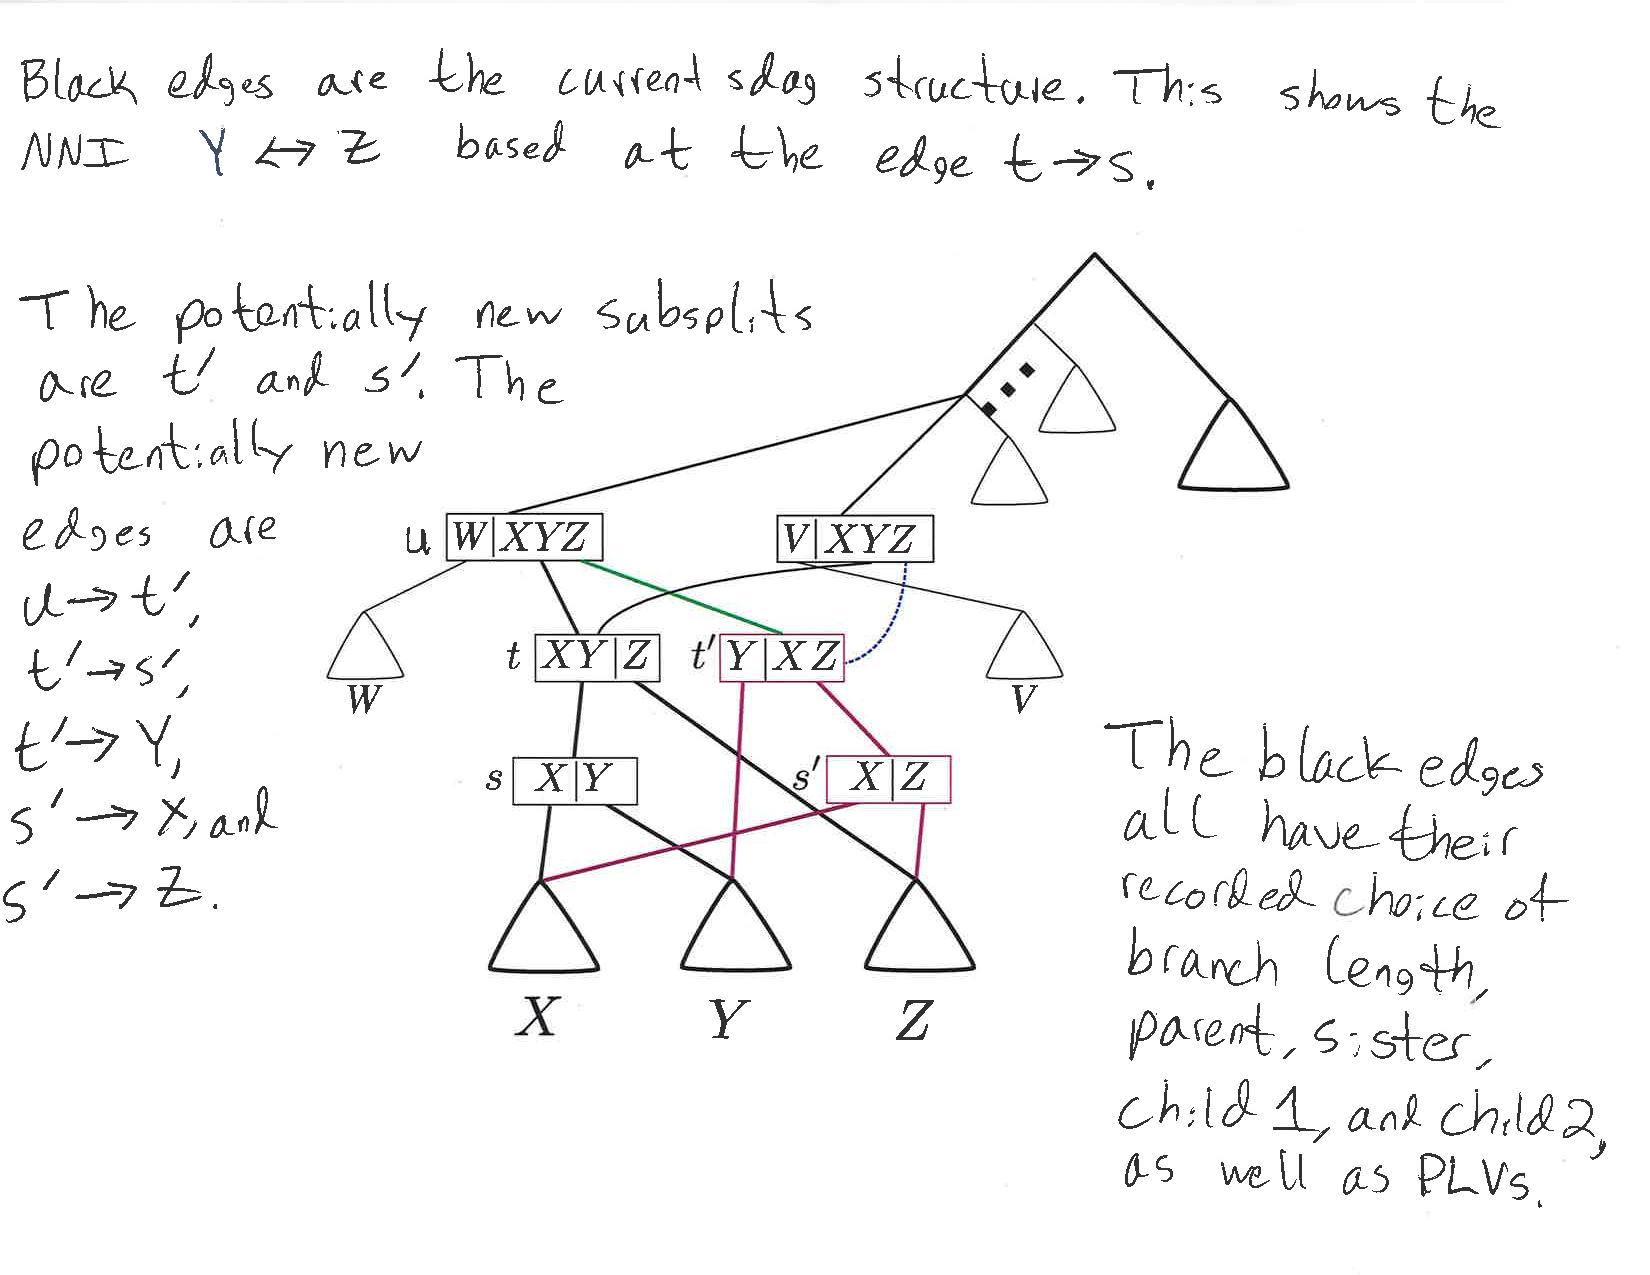
\includegraphics[scale=0.4]{figures/top_pruning_nni_labels.pdf}
\vspace{-3ex}
\caption{An sDAG, NNI, and associated edges. Note $X$, $Y$, and $Z$ are rooted sDAG sub-structures, not necessarily trees.
Parts of the sDAG in black indicate an existing sDAG with branch lengths and choice maps.
The edges in purple and green are the potentially new edges. The edge in blue is a parent edge not selected by the choice maps.
The existing choice maps take $\text{parent}(t\rightarrow s) = u\rightarrow t$, $\text{sibling}(t\rightarrow s) = t\rightarrow Z$, $\text{child}_1(t\rightarrow s) = s\rightarrow X$, and $\text{child}_2(t\rightarrow s) = s\rightarrow Y$.}
\label{fig:topPruningChoices}
\end{figure}

The top pruning algorithm is greedy. Suppose we given an sDAG $\mathcal{D}$ with choice maps and branch lengths, either from a single tree or list of trees.
\begin{enumerate}
\item Create a ranked list of NNIs and their likelihoods for each edge in the sDAG (two NNIs per sDAG edge). 
We do not record NNIs in the list if they do not enlarge $\mathcal{D}$.
\item Enlarge $\mathcal{D}$ to $\mathcal{D}^\prime$, with the highest likelihood NNI of the list, by adding
the new subsplits (at most two) and edges (at most five).
% CJS: @Dave, do we add any other edges in the current implementation? I recall you saying we do, which ones are they?
\item Remove the NNI of step 2 from the list. 
\item Insert into the list the NNIs and likelihoods of the new edges that enlarge $\mathcal{D}^\prime$.
\item Return to step 2 with $\mathcal{D}^\prime$ in place of $\mathcal{D}$.
\end{enumerate}
The repetition continues until either a set maximum number of iterations or the likelihoods of NNIs are all below a set threshold.


\subsection{Implementation of systematic search}

The necessary functionality for both NNI-searches are implemented in the Python-interface C++ library bito (\url{https://github.com/phylovi/bito}) and an interface to perform a search is further implemented in Python (\url{https://github.com/matsengrp/sdag-nni-experiments}).
Both generalized pruning and top pruning use partial likelihood vectors (PLVs) for fast and efficient likelihood calculations.
The partial likelihood vectors for top pruning are defined as usual for a two-pass version of Felsenstein's pruning algorithm and are propagated along the choice maps. 
The PLVs for generalized pruning follow a different pattern and are discussed in detail in \cite{GP}.

When new edges are introduced for top pruning, the optimization of associated branch lengths is done naively. 
We take one branch length, hold the others fixed, apply Brent optimization (maximizing the likelihood of the best known tree associated to the NNI), repeat with another branch length, and continue until values have approximately converged.
%CJS: @Dave Does GP do something different for branch lengths?


\subsection{Benchmarking setup}

The motivating question is, ``does the sDAG help us find additional trees in the topological posterior distribution?''
Necessarily the posterior density of topologies in an sDAG is at least that of the topologies used to construct the sDAG. 
But how much is the additional posterior density and how many additional topologies are in the sDAG? 
As part of benchmarking our systematic search algorithms, we calculate these numbers for an MCMC exploration of tree topologies.
Assume we have a ``golden run'' of a data set yielding a well-defined posterior on topologies.
Now starting from the beginning of an MCMC run on the data set, let $S$ be the set of topologies sampled after $k$ MCMC generations, $\mathcal{D}$ be the sDAG built from $S$, and $T$ be the set of topologies in $\mathcal{D}$.
How large are: the posterior density of trees in $S$, the posterior density of trees in $T$, $S$ relative to $T$, and $S \cap C$ relative to $T \cap C$, where $C$ is the $95\%$ credible set?
Rather than plotting these values against $k$, the number of generations, we use the number of distinct topologies found after $k$ generations.

We compute these values for the ds-datasets and plots are given in Figure \ref{fig:mcmc_to_sdag_stats}.
These data sets are multiple RNA sequence alignments commonly used to benchmark phylogenetic search methods.
Basic information for the data sets and their empirical posteriors is in Table \ref{table:dataSetStats}.
The empirical posteriors and credible sets assume the Jukes-Cantor substitution model and are determined by running Mr. Bayes for $10^{9}$ generations with 4 chains, uniform priors (topologies and branch lengths), sampling every 1000 generations, and discarding the first 10\% 
as burn-in. There is the ds2 data set. We omit this data set as the posterior is extremely diffuse and nearly flat, so MCMC methods yield an unreliable posterior.
While both of our search methods run on this data set, without an accurate estimate of the true posterior, we cannot measure the performance.

In all cases the number of topologies in the sDAGs quickly outpaces the number of input topologies. 
The gains in posterior density vary by data set, with the more diffuse posteriors yielding higher gains.
Since MCMC struggles to determine diffuse posteriors, using sDAGs may be beneficial.

\begin{figure}[!t]\centering
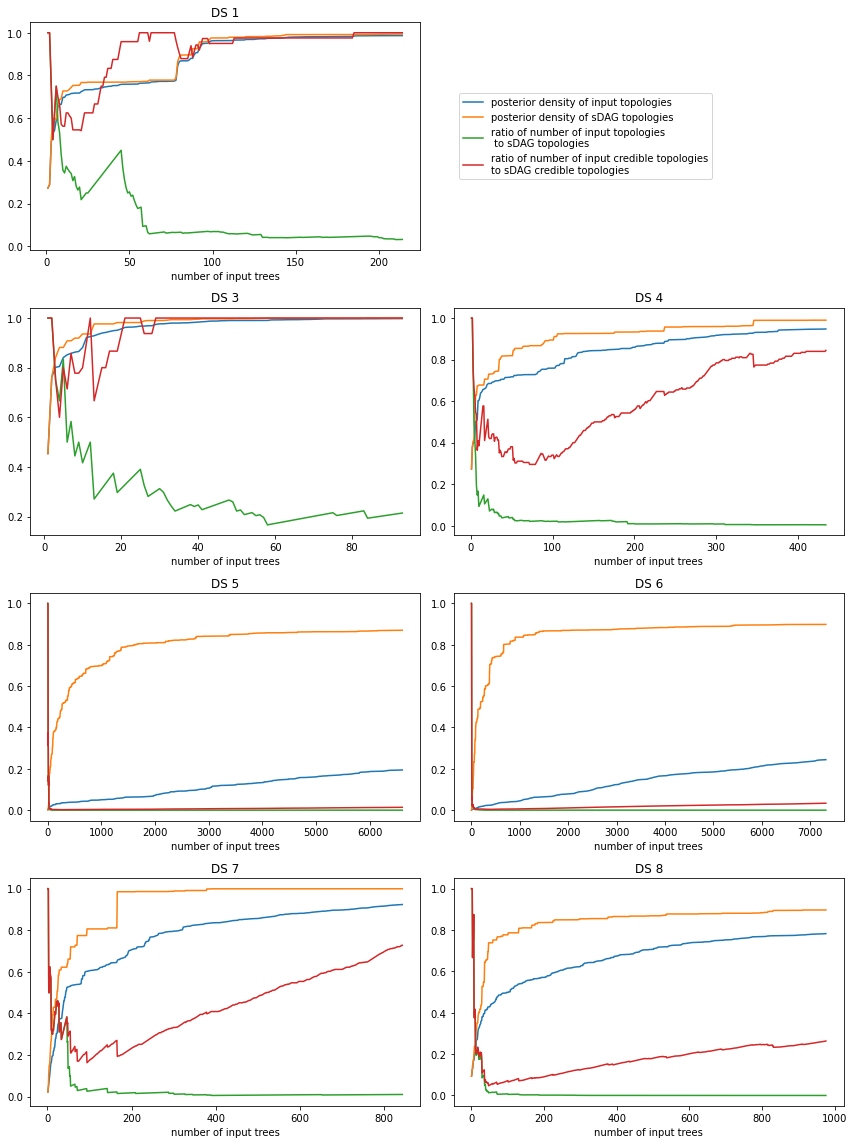
\includegraphics[scale=0.35]{figures/mcmc_sdag_stats.png}
\vspace{-1ex}
\caption{Topologies and spanned sDAGs from MCMC exploration of the ds-datasets. 
Input topologies are from running Mr. Bayes with the same specifications as the posterior, except for $10^{5}$ generations and initial tree set to the highest posterior density topology of the long run and branch lengths optimized by \iqtree.}
\label{fig:mcmc_to_sdag_stats}
\end{figure}

\begin{table}\centering
\begin{tabular}{ccccc}
&&& 95\% credible set & empirical posterior
\\
data set	& taxa & sites & topology count & topology count
\\\hline
1 & 27 & 1949 & 42 & 1245
\\\hline
3 & 36 & 1812 & 16 & 240
\\\hline
4 & 41 & 1137 & 219 & 4539
\\\hline
5 & 50 & 378 & 260894 & 298768
\\\hline
6 & 50 & 1133 & 157942 & 195816
\\\hline
7 & 59 & 1824 & 756 & 6000 
\\\hline 
8 & 64 & 1008 & 4329 & 26442
\end{tabular}
\caption{ds-datasets}
\label{table:dataSetStats}
\end{table}

We ask the same questions of our systematic search algorithms. How much of the posterior is captured per iteration and how unnecessarily large are the sDAGs? The answers to these questions are in the next section. 


\section{Results}

The experiments of this section can be recreated by following the instructions in the experiments Github repository (\url{https://github.com/matsengrp/sdag-nni-experiments}).

Figure \ref{fig:generalizedPruningFoundPosterior} shows the performance of generalized pruning in terms of the posterior density of found topologies,
while Figure \ref{fig:topPruningFoundPosterior} contains the equivalent plots for top pruning.
We compare against MCMC by taking topologies from short runs of Mr. Bayes, as in figure \ref{fig:mcmc_to_sdag_stats}, and match the results on the number of likelihood calculations.
The initial sDAG for each nni-search is given by the highest posterior topology of the empirical posterior with branch lengths determined by \iqtree\, (i.e., generalized pruning, top pruning, and short MCMC start with the same tree).

\vspace{-8ex}
\begin{figure}[!b]\centering
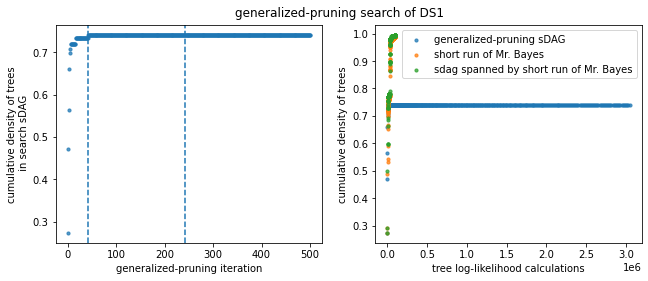
\includegraphics[scale=0.4]{figures/gp_ds1_pp.png}
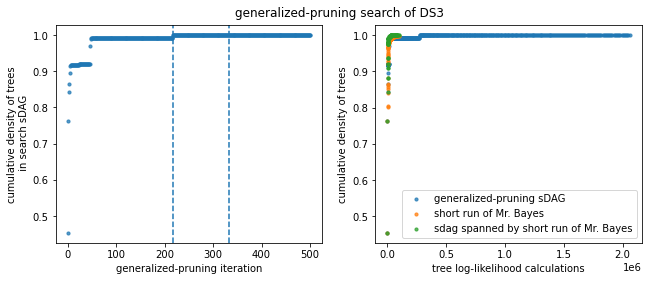
\includegraphics[scale=0.4]{figures/gp_ds3_pp.png}
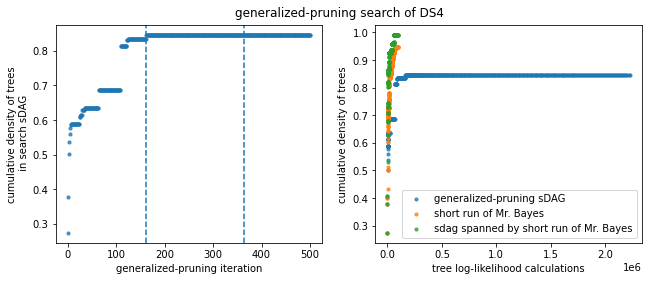
\includegraphics[scale=0.4]{figures/gp_ds4_pp.png}
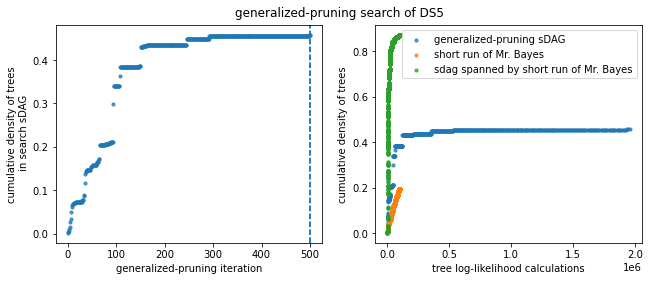
\includegraphics[scale=0.4]{figures/gp_ds5_pp.png}
\clearpage
\end{figure}
\begin{figure}[!t]\centering
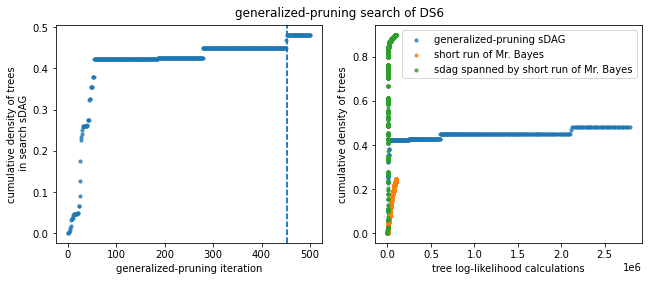
\includegraphics[scale=0.4]{figures/gp_ds6_pp.png}
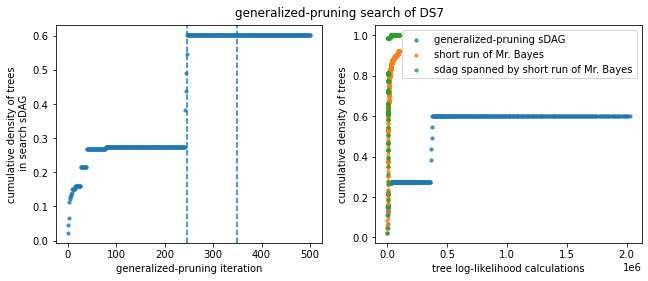
\includegraphics[scale=0.4]{figures/gp_ds7_pp.png}
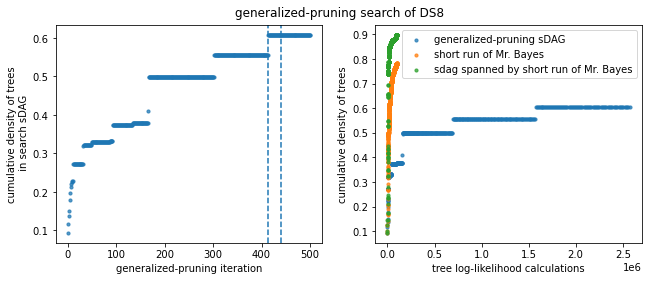
\includegraphics[scale=0.4]{figures/gp_ds8_pp.png}
\caption{The empirical posterior density found by generalized pruning on the ds-datasets and a comparison with MCMC.
The dashed blue lines indicate the last iteration finding a topology of the credible set and the last iteration finding a topology of the empirical posterior. 
The empirical posteriors are the same as in Figure \ref{fig:mcmc_to_sdag_stats}.}
\label{fig:generalizedPruningFoundPosterior}
\end{figure}

\vspace{8ex}
Generalized pruning kind of sucks... 
Let's double check we're calculating the right things in the search.
Either we can do better or this really is the performance and we can say something about that.


Top pruning consistently outperforms the topologies of a short MCMC run and often outperforms the sDAG spanned by these topologies.
We point out that the sDAG spanned by topologies of the short MCMC runs is not part of any implementation. 
Instead it represents the sDAG information one could extract from those topologies.
Simply generating these sDAGs from MCMC runs would not give an efficient algorithm.

\begin{figure}[!b]\centering
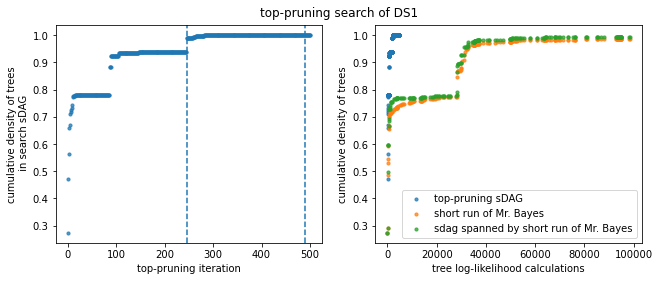
\includegraphics[scale=0.4]{figures/tp_ds1_pp.png}
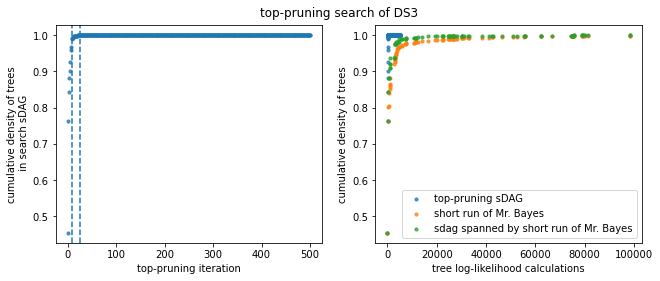
\includegraphics[scale=0.4]{figures/tp_ds3_pp.png}
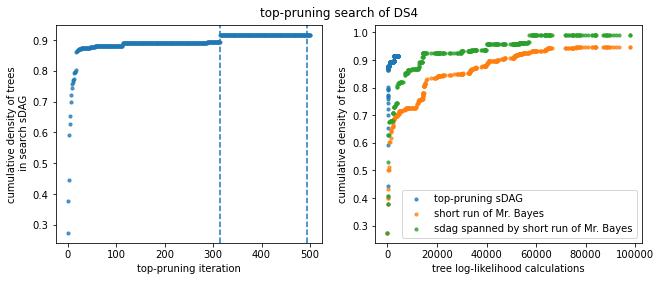
\includegraphics[scale=0.4]{figures/tp_ds4_pp.png}
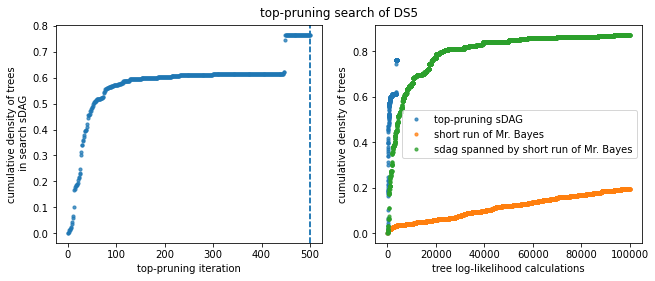
\includegraphics[scale=0.4]{figures/tp_ds5_pp.png}
\end{figure}
\begin{figure}[!t]\centering
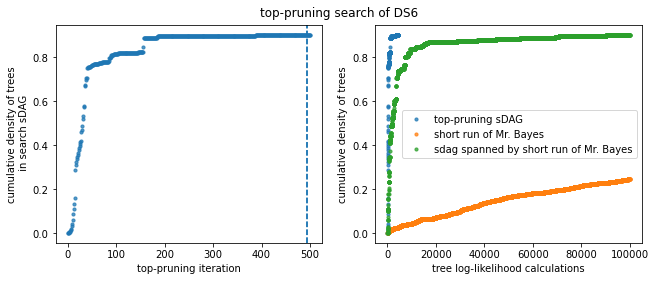
\includegraphics[scale=0.4]{figures/tp_ds6_pp.png}
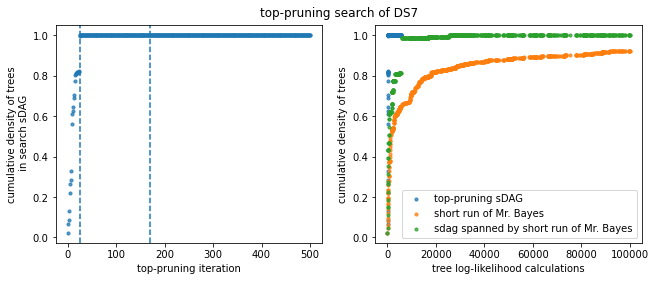
\includegraphics[scale=0.4]{figures/tp_ds7_pp.png}
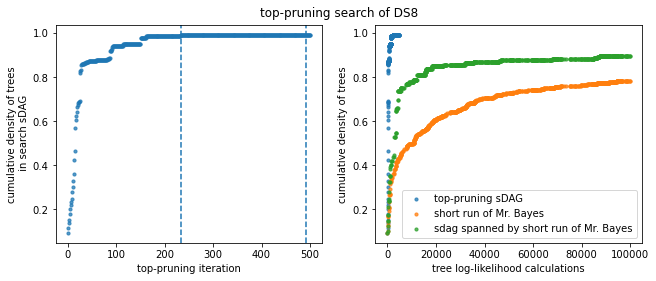
\includegraphics[scale=0.4]{figures/tp_ds8_pp.png}
\caption{The empirical posterior density found by top pruning on the ds-datasets and a comparison with MCMC.
The dashed blue lines indicate the last iteration finding a topology of the credible set and the last iteration finding a topology of the empirical posterior. 
The empirical posteriors are the same as in Figure \ref{fig:mcmc_to_sdag_stats}.}
\label{fig:topPruningFoundPosterior}
\end{figure}


Comparing the number of likelihood calculations of one method to another can be problematic, since Mr. Bayes uses local rearrangements of topologies and reuses calculations. 
Here it is a somewhat fair comparison because the likelihood calculations of generalized pruning and top pruning use 
rootward and leafward partial likelihood vectors on the sDAG, so the calculations are also local and reused.
We would like to compare by actual run-time.  
Right now the run-time of top-pruning is not linear in the number of iterations, but it will be soon...
%CJS: I'll fill this in when Dave is finished and I've reran the timing scripts.
On diffuse subsets, top-pruning does not witness the 95\% credible set within 500 iterations, which would be good to address...
%CJS: What can we say about it right now?

The plots of Figures \ref{fig:generalizedPruningCounts} and \ref{fig:topPruningCounts} show the extent generalized and top-pruning select good edges, which increase
the found posterior, versus those that instead unnecessarily enlarge the sDAG. 
In the ideal setting, the search methods would only add edges present in the posterior.

\vspace{-2.3ex}
\begin{figure}[!hb]\centering
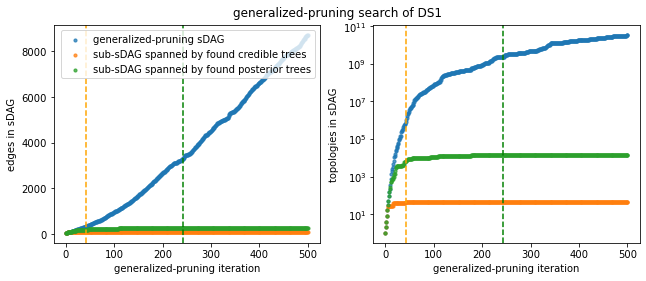
\includegraphics[scale=0.4]{figures/gp_ds1_counts.png}
\vspace{-1.2ex}
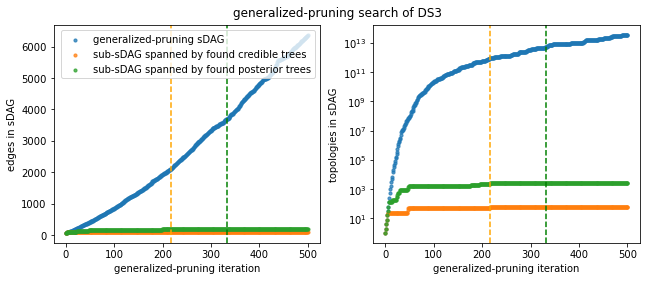
\includegraphics[scale=0.4]{figures/gp_ds3_counts.png}
\vspace{-1.2ex}
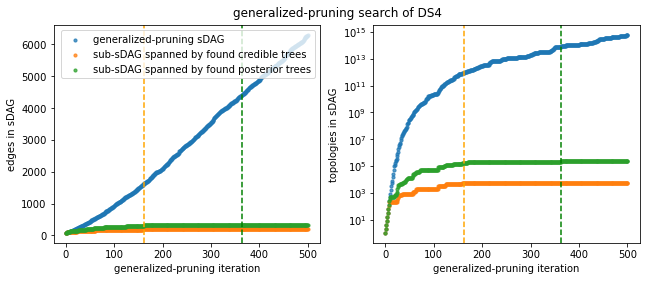
\includegraphics[scale=0.4]{figures/gp_ds4_counts.png}
\vspace{-1.2ex}
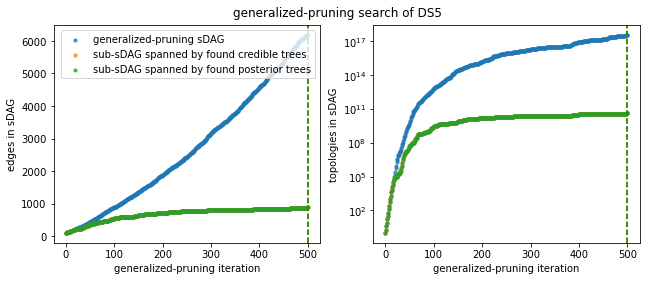
\includegraphics[scale=0.4]{figures/gp_ds5_counts.png}
\vspace{-1.2ex}
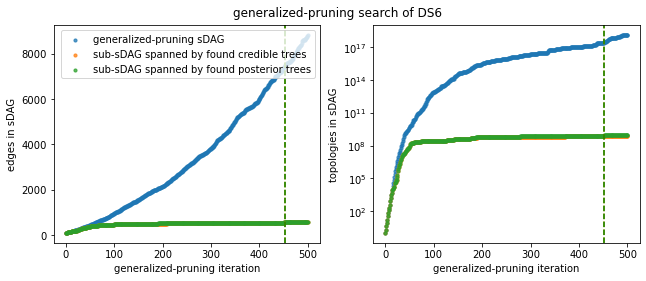
\includegraphics[scale=0.4]{figures/gp_ds6_counts.png}
\end{figure}
\begin{figure}[!t]\centering
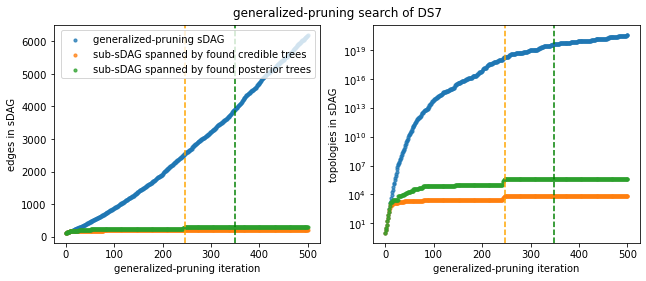
\includegraphics[scale=0.4]{figures/gp_ds7_counts.png}
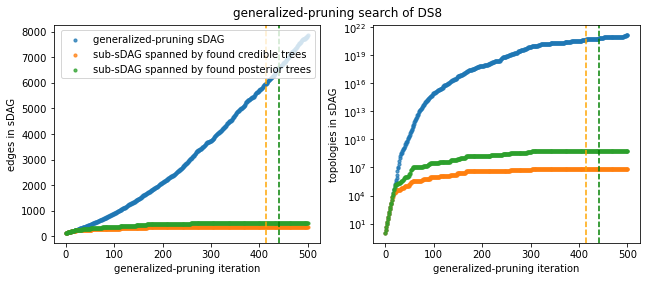
\includegraphics[scale=0.4]{figures/gp_ds8_counts.png}
%\vspace{-3ex}
\caption{The number of edges and topologies in the sDAGs constructed by top-pruning.
The dashed orange lines indicate the last iteration finding a topology of the credible set, the dashed green lines indicate the last iteration finding a topology of the empirical posterior. }
\label{fig:generalizedPruningCounts}
\end{figure}


\begin{figure}[!b]\centering
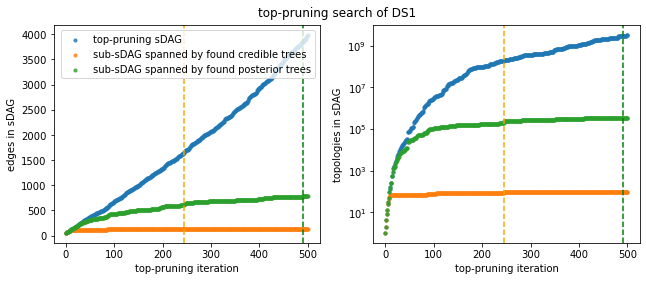
\includegraphics[scale=0.4]{figures/tp_ds1_counts.png}
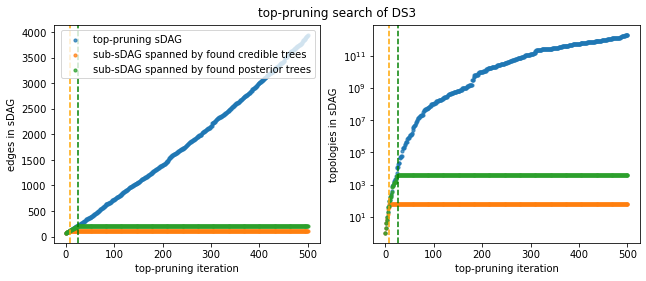
\includegraphics[scale=0.4]{figures/tp_ds3_counts.png}
\end{figure}
\begin{figure}[!t]\centering
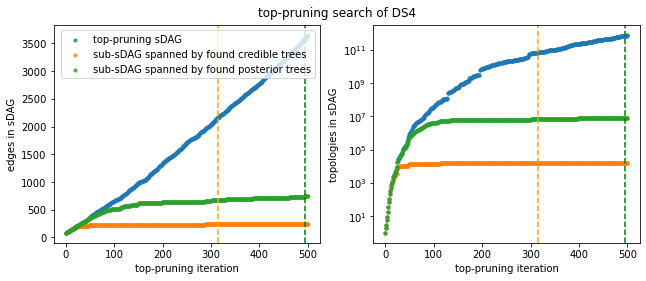
\includegraphics[scale=0.4]{figures/tp_ds4_counts.png}
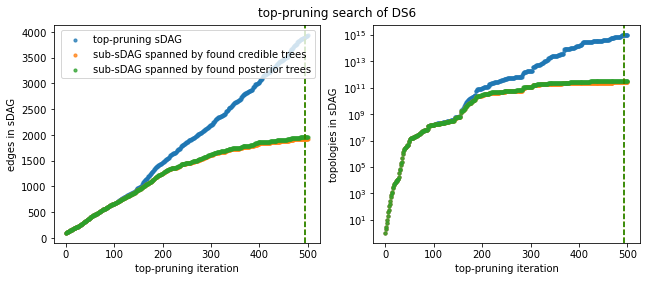
\includegraphics[scale=0.4]{figures/tp_ds6_counts.png}
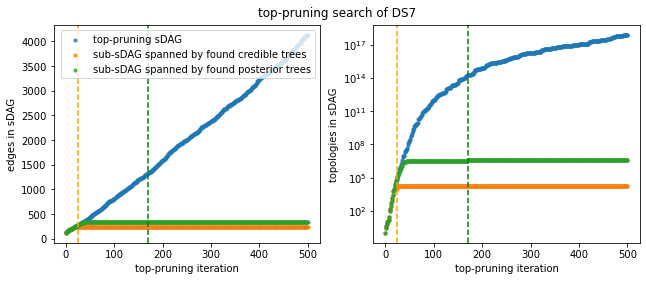
\includegraphics[scale=0.4]{figures/tp_ds7_counts.png}
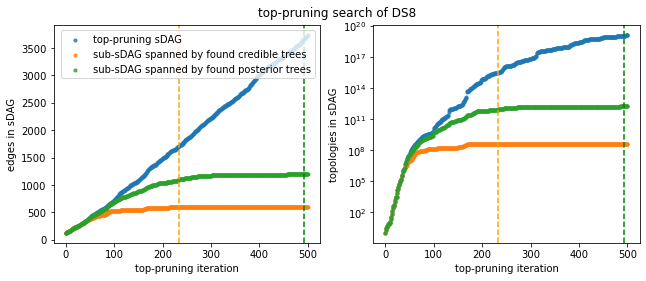
\includegraphics[scale=0.4]{figures/tp_ds8_counts.png}
%\vspace{-3ex}
\caption{The number of edges and topologies in the sDAGs constructed by top-pruning.
The dashed orange lines indicate the last iteration finding a topology of the credible set, the dashed green lines indicate the last iteration finding a topology of the empirical posterior. }
\label{fig:topPruningCounts}
\end{figure}
\clearpage



\section{Discussion}


While top pruning performs well on our test data sets, the number of sequences is relatively small, with 64 being the largest. 
We do not yet know how well top pruning scales to larger data sets, where we have thousands or tens of thousands of sequences.
Our current method of benchmarking is not possible for such data sets, as we require an empirical estimate of the true posterior.

GP is doing worse, is there anything to do for it?

One could imagine extensions allowing more general additions to the sDAG in our search algorithms.
When proposing and ranking NNIs, we could try edges other than those present in the choice maps.
For example, rather than using the parent of $t$ specified in the choice map, we could try the other edges from $t$ as candidate parents for $t^{\prime}$ (such as the blue edge in Figure \ref{fig:topPruningChoices}).
This requires only a little extra evaluation and branch length optimization.
Note that if we use one of these alternate edges, the resulting modification is no longer an NNI in the strict sense, as the trees using the new edge will be more different than one NNI away from any tree using the previous edge.

Furthermore, when we add the best NNI to the sDAG and remove it from the ranked list, some of the NNIs in the list may now have an edge present in the current sDAG that was not present before. Such an edge has a branch length and choice maps that may yield a different likelihood from before. In such cases, 
we could trigger re-optimization of branch lengths for that NNI and replacing the corresponding likelihoods, PLVs, and choice maps.














\bibliographystyle{abbrv}
\bibliography{main}




\end{document}
